\documentclass[conference]{IEEEtran}
\IEEEoverridecommandlockouts

% Packages
\usepackage{cite}
\usepackage{amsmath,amssymb,amsfonts}
\usepackage[dvipsnames]{xcolor}
\usepackage{graphicx}
\usepackage{textcomp}
\usepackage{listings}
\usepackage{subcaption}
\usepackage{multirow}
\usepackage{algorithm}
\usepackage{algpseudocode}
\usepackage{algorithmicx}
\usepackage{url}
\usepackage{caption}
\usepackage{tcolorbox}
\usepackage{hyperref}
\usepackage[T1]{fontenc}
\usepackage{enumitem}
\usepackage{multicol}
\usepackage{enumitem}
\usepackage{balance}

\setlength {\marginparwidth }{2cm}

\hypersetup{hidelinks}
\newcommand{\algorithmautorefname}{Algorithm}
\captionsetup[algorithm]{name=Alg.} 

\tcbuselibrary{listingsutf8}
\newtcbox{\redbox}[1][]{
 on line, 
 boxsep=1pt, 
 left=1pt, 
 right=1pt, 
 top=1pt, 
 bottom=1pt, 
 colframe=red!75!black, 
 colback=red!10, 
 boxrule=0.5pt, 
 rounded corners,
 #1
}

\algrenewcommand\algorithmicindent{0.8em} 

\hyphenation{GROMACS}
\hyphenation{LAMMPS}
\hyphenation{ls1 mardyn}
\hyphenation{AutoPas}


\begin{document}

\title{Algorithm Selection and Auto-Tuning in AutoPas}

\author{
    \IEEEauthorblockN{ Manuel Lerchner}
    \IEEEauthorblockA{
        \textit{Technical University of Munich}\\
        Munich, Germany}
}

\maketitle

\begin{abstract}
    Simulating molecular dynamics (MD) presents a significant computational challenge due to the vast number of particles involved in modern experiments. Naturally, researchers have put much effort into developing algorithms and frameworks that can efficiently simulate these systems. This paper focuses on the AutoPas framework, a modern particle simulation library that uses dynamic optimization techniques to achieve high performance in complex simulation scenarios. We compare AutoPas with other prominent MD engines, such as GROMACS, LAMMPS, and ls1 mardyn, and investigate a possible improvement to AutoPas' auto-tuning capabilities by introducing an early stopping mechanism aiming to reduce the overhead of parameter space exploration. Our evaluation shows that such a mechanism can reduce the total simulation time by up to 18.9\% in specific scenarios, demonstrating the potential of this improvement.
\end{abstract}

\begin{IEEEkeywords}
    molecular dynamics, auto-tuning, AutoPas, early-stopping, GROMACS, LAMMPS, ls1 mardyn
\end{IEEEkeywords}

\section{Introduction}

Molecular dynamics simulations represent a computational cornerstone in various scientific fields. These simulations typically use complex and computationally intensive interaction models acting on enormous numbers of particles to ensure accurate results. Consequently, the computational requirements for these simulations can be substantial and require highly optimized algorithms and frameworks to achieve feasible performance.

Well-established molecular dynamics engines, such as GROMACS, LAMMPS, and ls1 mardyn, solve this challenge by providing a single, highly optimized implementation determined before the start of the simulation. As their implementation is determined statically, these engines must rely on static optimizations to improve their performance. Static optimizations are typically selected based on predefined performance models and must be fine-tuned for specific hardware architectures. Common static optimization techniques include automatic optimizations performed by modern compilers (e.g., loop unrolling, inlining, auto-vectorization), conditional compilation based on the target hardware (e.g., SIMD), or manual selection of simulation parameters based on expert knowledge~\cite{Gratl2019AutoPas}.

AutoPas approaches the challenge of high-performance molecular dynamics simulations differently: Instead of choosing a single implementation prior to the simulation, AutoPas uses dynamic optimizations to adjust its implementation based on the simulation state and the actual hardware performance. This approach is favorable, as the engine can adapt and optimize itself without external intervention. However, dynamic optimizations come at the cost of increased complexity and potential overhead due to the need for frequent re-evaluations of the selected implementation.

This paper provides an overview of the AutoPas framework and the benefits and challenges of using dynamic auto-tuning in molecular dynamics simulations. We compare AutoPas with other prominent MD engines, such as GROMACS, LAMMPS, and ls1 mardyn, and investigate a possible improvement to AutoPas' auto-tuning capabilities by introducing an early stopping mechanism aiming to reduce the overhead of parameter space exploration.

\section{AutoPas}

AutoPas was developed on the basis of creating an efficient node-level particle simulation engine applicable to a wide range of scientific fields~\cite{Tchipev2020}. To achieve this goal, AutoPas uses a modular architecture that seamlessly integrates different algorithms and data structures into the simulation engine. As it is not capable of running simulations on its own, AutoPas serves as an intermediary layer between user-provided simulation code and implementations specifically designed to efficiently solve N-Body problems. The modular nature of AutoPas enables it to combine different implementations and create a wide range of so-called \textit{configurations}.

To eliminate the need for manual configuration selection and enable dynamic optimization, AutoPas provides an auto-tuning framework. This framework periodically assesses different configurations and selects optimal ones based on performance metrics. This selection process is managed by \textit{TuningStrategies} that systematically suggest promising configurations to evaluate. \autoref{fig_architecture} illustrates the high-level architecture of the AutoPas library.

\begin{figure}[H]
    \centering
    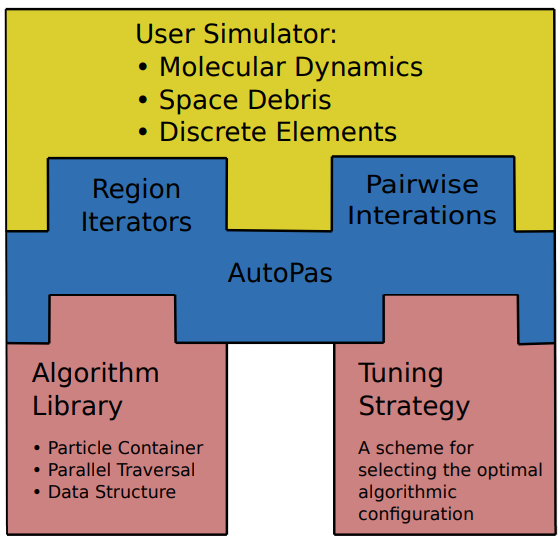
\includegraphics[width=2.2in]{figures/AutoPasLibraryStructure.png}
    \caption{AutoPas Library Structure as depicted by~\cite{Newcome2023Poster}}
    \label{fig_architecture}
\end{figure}

\subsection{Algorithm Library}

All different algorithmic implementations for solving N-Body problems are part of the so-called \textit{Algorithm Library} of AutoPas. The Algorithm Library contains different implementations for certain key aspects of the simulation, such as neighbor identification, traversal patterns, memory layouts, and optimization techniques. Currently, AutoPas supports the six tunable parameters: \textit{Container}, \textit{Data Layout}, \textit{Newton 3}, \textit{Traversal}, \textit{Load Estimator} and \textit{Cell Size Factor} which combine to form a configuration.

Maintaining a library of different implementations has several benefits: As the library is modular, it is straightforward to add new, potentially hardware-specific, implementations for each key aspect of the simulation. This ensures that the simulation engine remains maintainable and can provide performance portability across a wide range of hardware platforms~\cite{Tchipev2020}. The interchangeable nature of the implementations also ensures implicit backward compatibility, making it easy to study the effects of new hardware on existing implementations~\cite{Tchipev2020}. Users of the library also benefit from this approach. As AutoPas is able to automatically select the best configuration for their specific use case and hardware setup, users do not need to have a deep understanding of the underlying hardware or software optimizations and can fully focus on the high-level aspects of their simulation~\cite{Tchipev2020}\cite{Gratl2022AutoPas}.

\subsection{Tunable Parameters}

This section provides a brief overview of the six tunable parameters available in AutoPas.

\begin{description}[style=nextline]
    \item[Container]
        Containers are responsible for storing the simulation particles so that relevant neighbor particles can be determined efficiently. As AutoPas focuses on short-range interactions with a force cutoff radius $r_c$, efficient neighbor identifications using just $O(N)$ distance calculations are possible~\cite{Gratl2019AutoPas}. The container types depicted in \autoref{fig_containers} will be shortly described below.

        \begin{description}[style=nextline, font=\itshape]
            \item[$\bullet$ Linked Cells]
                The Linked Cells algorithm maintains a grid of cells, each storing a list of particles located within the cell. When calculating forces for a particle, only\footnote{If $cellSizeFactor = {cellSize}/{r_c} = 1$.} particles in neighboring cells (depicted in blue) must be considered, as all other particles are guaranteed to be outside the cutoff radius.

                LinkedCells introduces many spurious distance calculations (shown by arrows to gray particles), which can be reduced by using a smaller cell size factor~\cite{menges2019}. LinkedCells are very cache-friendly as spatially close particles are stored together in memory~\cite{Gratl2022AutoPas}.

            \item[$\bullet$ Verlet Lists]
                The Verlet Lists algorithm uses a second radius $r_v = {r_c} + \Delta_s$ (yellow circle) and considers all particles within this radius as potential neighbors. Contrary to LinkedCells, each particle maintains its own list of potential neighbors, resulting in a higher memory overhead.
                As the bigger radius $r_v$ provides a buffer region, it is possible to only rebuild the neighbor-list every $n$ simulation steps, as long as no particle can move from outside $r_c + \Delta_s$ to inside $r_c$ unnoticed~\cite{NEWCOME2023115278}.

                VerletLists have few spurious distance calculations but are less cache-friendly as neighboring particles are not stored together in memory~\cite{Gratl2022AutoPas}. This results in very inefficient vectorization~\cite{PALL20132641}.

            \item[$\bullet$ Verlet Cluster Lists]
                The Verlet Cluster Lists algorithm improves on the VerletLists algorithm by grouping particles into clusters of size $M$ ($M=4$ in the figure) and performing neighbor-list calculations on a cluster level~\cite{PALL20132641}. This reduces the memory overhead significantly. However, it results in more spurious distance calculations as all particles in neighboring clusters must be considered when calculating forces. When $M$ is chosen in accordance with the SIMD width of the system, efficient vectorization is possible~\cite{Gratl2022AutoPas}~\cite{PALL20132641}.
        \end{description}

        \begin{figure}[h]
            \centering
            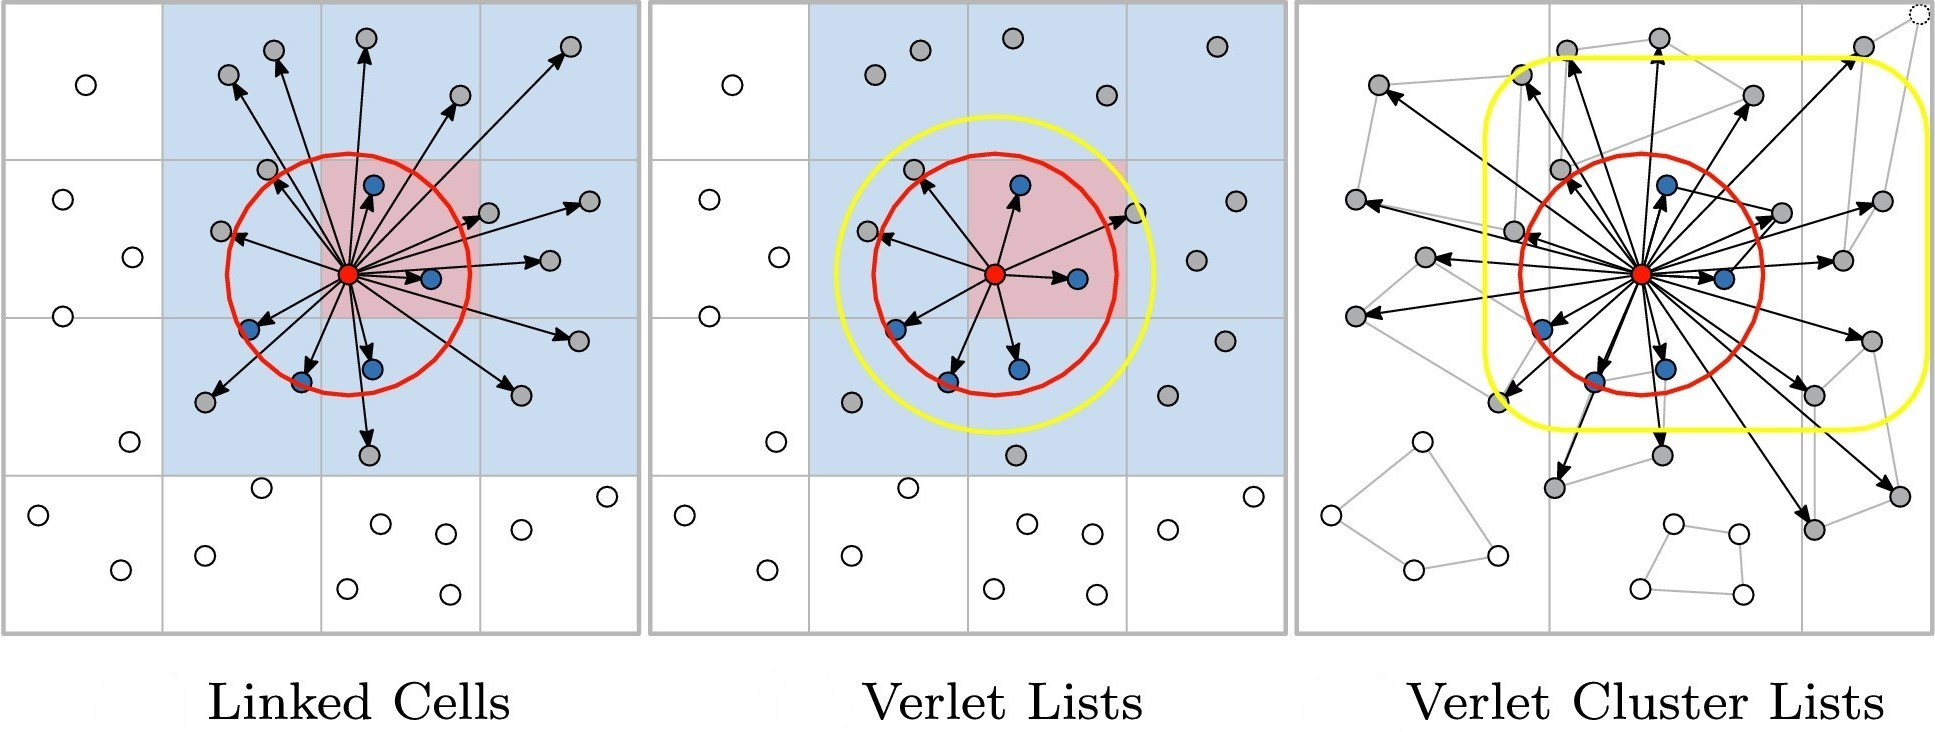
\includegraphics[width=\columnwidth]{figures/containers.jpg}
            \caption{Important container types as depited by~\cite{Gratl2022AutoPas}. The cutoff radius $r_c$ is shown using a red circle. Arrows represent distance checks between particles. Only particles shown in blue contribute to the final force calculation.}
            \label{fig_containers}
        \end{figure}

    \item[Data Layout]
        The Data Layout describes how the particles are stored in memory. Possible choices are \textit{SoA} (Structure of Arrays) and \textit{AoS} (Array of Structures). \textit{SoA} allows for better vectorization as properties of multiple particles can be loaded efficiently into SIMD registers. However, accessing the properties of a single particle is more expensive, requiring
        multiple memory accesses. \textit{AoS} is the opposite. It allows for efficient access to properties of a single particle to, e.g., send it to another MPI rank, but results in inefficient vectorization~\cite{Gratl2022AutoPas}.

    \item[Newton 3]
        A common optimization in molecular dynamics simulations is the application of Newton's third law, which allows reusing force calculations between two particles, reducing the number of force calculations by a factor of two. As Newton 3 can cause race conditions in parallel environments, not all traversal patterns support this optimization. The optimization can be enabled or disabled in accordance with the traversal pattern and the interaction model.

    \item[Traversal]
        Traversals are responsible for iterating over the particles in the simulation and calculating their interactions in a shared-memory environment~\cite{SECKLER2021101296}. The traversal pattern determines to which extent force calculations can be parallelized and whether optimizations, such as Newton 3, can be applied. The traversal patterns depicted in \autoref{fig_traversals} will again be shortly introduced below.

        \begin{description}[style=nextline, font=\itshape\mdseries]
            \item[$\bullet$ C01]
                The C01 traversal pattern processes each cell independently, resulting in an embarrassingly parallel traversal. Newton's Third Law cannot be used with this traversal pattern since adjacent cells are processed simultaneously, which could lead to race conditions when applying forces. As no synchronization between cells is required, the C01 traversal pattern has the highest degree of parallelism~\cite{NEWCOME2023115278}.
            \item[$\bullet$ C18]
                The C18 traversal pattern uses color assignments to ensure that no race conditions occur when using Newton 3. \autoref{fig_traversals} shows the regular color assignments, ensuring that no two cells of the same color share common neighbors. To ensure that forces are only applied once when using Newton 3, each cell only applies forces to cells \textit{above} or \textit{right} of it. During the force calculation, all available threads work on a single color, which allows for a safe application of forces on neighboring cells and reduces scheduling overhead~\cite{NEWCOME2023115278}. As the color groups must be processed sequentially, the C18 traversal introduces 18 synchronization points, which reduces the overall degree of parallelism\cite{NEWCOME2023115278}.

            \item[$\bullet$ C08]
                The C08 traversal pattern is similar to the C18 traversal pattern but uses a different coloring scheme with only eight colors, reducing the number of synchronization points to eight. The C08 traversal pattern has a degree of parallelism between the C01 and C18 traversal patterns~\cite{NEWCOME2023115278}.
        \end{description}

        \begin{figure}[H]
            \centering
            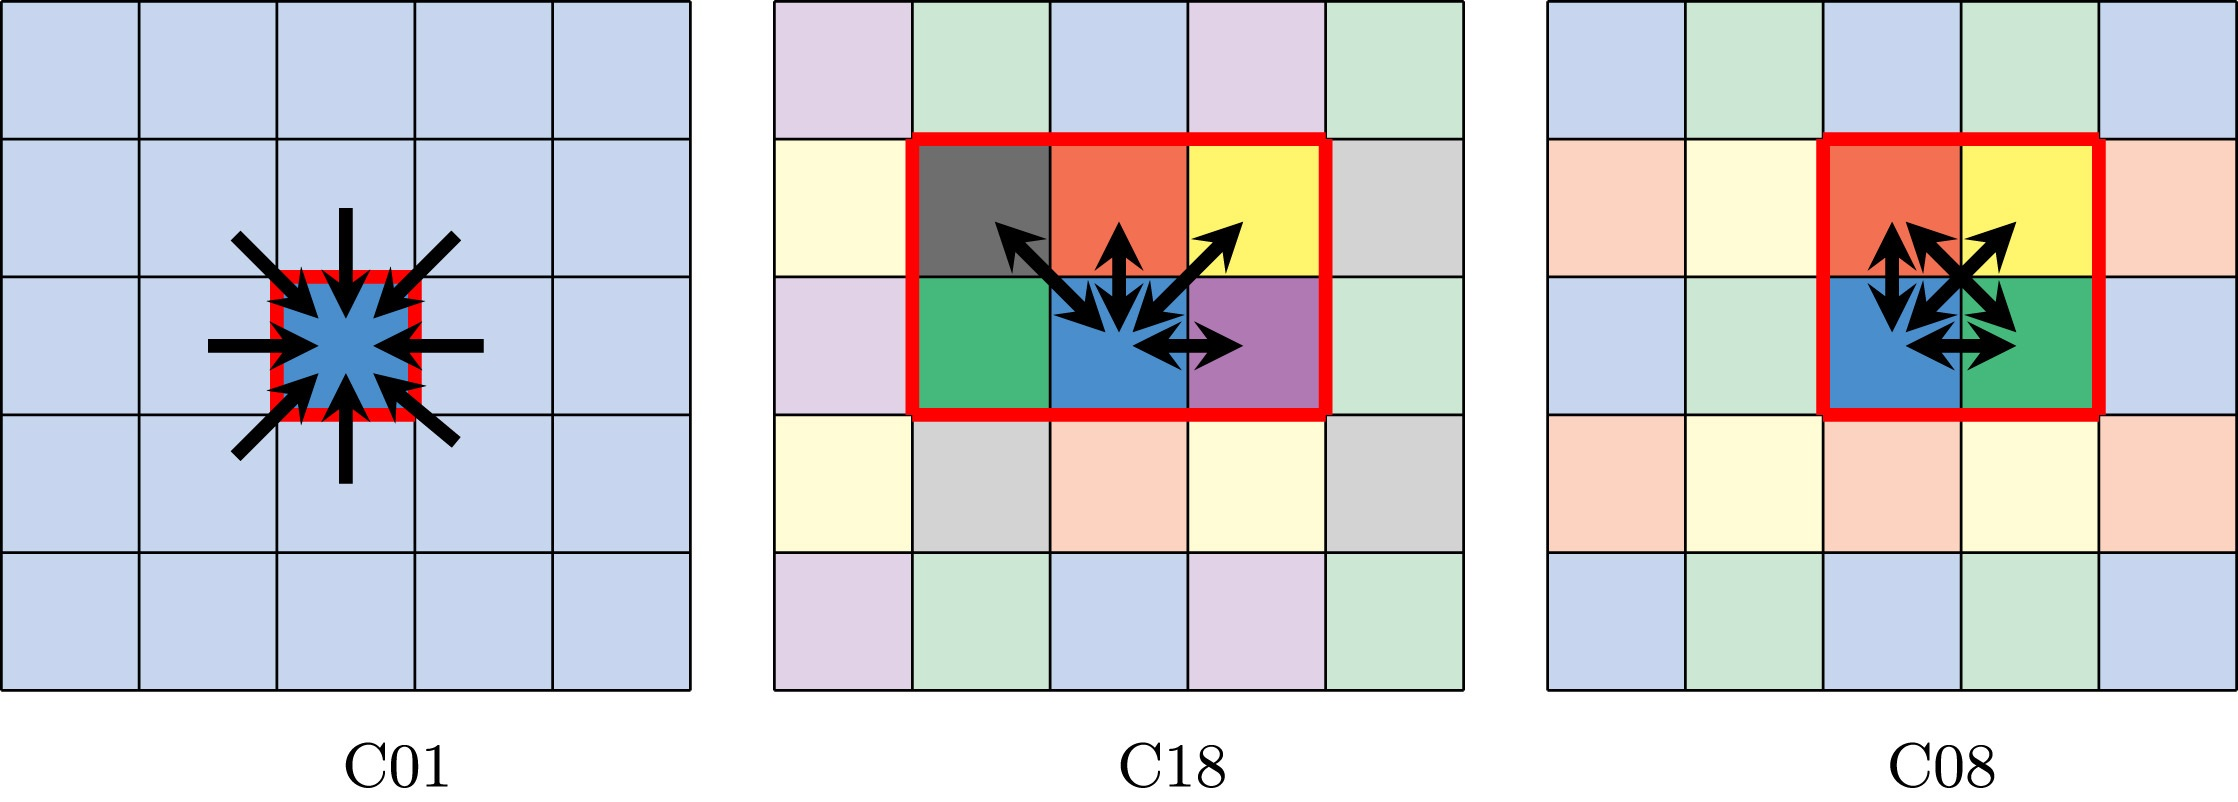
\includegraphics[width=\columnwidth]{figures/traversals.jpg}
            \caption{Important Traversal Types as depicted by~\cite{NEWCOME2023115278}.}
            \label{fig_traversals}
        \end{figure}

    \item[Load Estimator]
        Different load estimators can be used to estimate and fairly divide work across all available processing units. Maintaining a good workload distribution reduces the idle time of processing units and thus increases the overall simulation speed.

    \item[Cell Size Factor]
        The default cell size factor of 1 results in a cell size of $r_c$ (see \autoref{fig_containers}). As discussed previously, the large area of neighboring cells causes many spurious distance calculations, which can be reduced by using a smaller cell size factor. As decreasing the cell size factor also increases the memory overhead due to the higher number of cells to be maintained in memory~\cite{menges2019}~\cite{Papula2020}, the cell size factor must be chosen carefully.
\end{description}


\subsection{Auto-Tuning Framework}

A manual selection of suitable implementations for each tunable parameter would require extensive domain knowledge that is challenging to acquire and maintain under the constantly changing software and hardware landscape. To address this issue, AutoPas performs automated algorithm selection to optimize specific performance metrics, such as simulation speed or energy efficiency~\cite{Gratl2022AutoPas}. Internally, AutoPas periodically initiates so-called \textit{tuning-phases} in which promising configurations are evaluated in order to determine the best configuration for the current simulation state. The winning configuration is then used until the next tuning phase is initiated.

The key to efficient tuning phases is the ability to efficiently determine promising configurations. The naive approach of evaluating all possible configurations is infeasible in practice, as many configurations turn out to be orders of magnitude slower than the optimal configuration~\cite{endreport.pdf}\cite{Manuel_Lerchner_Thesis.pdf}.

AutoPas attempts to mitigate this problem by using Tuning Strategies. Tuning strategies inspect prior timing measurements or the simulation state and try to infer which configurations are likely to perform well. Only those configurations will then be evaluated.

The currently available tuning strategies in AutoPas are:

\begin{description}[style=nextline]
    \item[FullSearch]
        The FullSearch strategy naively evaluates all possible configurations, thus always finding the best configuration. As many configurations tend to be suboptimal\cite{Manuel_Lerchner_Thesis.pdf}, the FullSearch strategy often causes a considerable overhead.

    \item[RandomSearch]
        The RandomSearch strategy randomly selects configurations out of the entire search space, causing less overhead than the FullSearch strategy at the cost of potentially missing the best configuration.

    \item[BayesianSearch]
        The Bayesian Search strategy is similar to the RandomSearch strategy. However, it uses a Bayesian optimization algorithm to select the next configuration to evaluate based on previous measurements~\cite{njan_master}. An improvement to better account for the discrete tuning space of AutoPas called \textit{BayesianClusterSearch} is also available~\cite{njan_master}.

    \item[PredictiveTuning]
        The PredictiveTuning strategy extrapolates previously gathered timing measurements of a configuration to predict its performance in the current simulation state. This allows for an efficient rejection of inefficient configurations without evaluating them~\cite{pelloth2020}.

    \item[RuleBasedTuning]
        The RuleBasedTuning strategy uses a set of rules to discard undesirable configurations immediately. The rules are based on expert knowledge in a \textit{if-then} fashion and use aggregate statistics of the simulation state to make decisions~\cite{endreport.pdf}.

    \item[FuzzyTuning]
        The FuzzyTuning strategy is similar to the RuleBasedTuning strategy but uses fuzzy logic systems to evaluate configurations. This allows for both an inter- and extrapolation of the rules to account for configurations not covered by the expert knowledge~\cite{Manuel_Lerchner_Thesis.pdf}.

\end{description}

\section{Benefits of Auto-Tuning}

Since no single configuration can deliver optimal performance across all simulation scenarios~\cite{Tchipev2020}, dynamic performance tuning is essential for maintaining high efficiency across diverse simulation conditions. This section discusses some of the key benefits of using AutoPas's auto-tuning framework.

\subsection*{Performance Improvements}

The most compelling advantage of auto-tuning is the significant performance improvements it can achieve. It has been shown many times that AutoPas can improve simulation times across diverse molecular dynamics simulation scenarios, both in the standalone application as well as in established MD engines such as ls1 mardyn and LAMMPS~\cite{SECKLER2021101296}\cite{Gratl2022AutoPas}. Those improvements provide compelling evidence for the effectiveness and importance of the auto-tuning approach.

\subsection*{Accessibility and Ease of Use}

AutoPas's tuning framework enables users to achieve optimal performance directly out of the box without requiring deep expertise in performance optimization. The inherent user-friendliness is particularly valuable when integrating AutoPas into other simulation frameworks, as developers can treat the simulation engine as a black box and let the auto-tuning framework handle the optimization.

\section{Drawbacks of AutoTuning}

\subsection*{Suboptimal Configurations}

A major drawback of auto-tuning in the way it is implemented in AutoPas is the inherent overhead caused by tuning phases. As the tuning process requires evaluating many configurations, the overhead of configurations, performing orders of magnitude worse than the optimal configuration, quickly leads to noticeable increases in the total simulation time~\cite{endreport.pdf}~\cite{Manuel_Lerchner_Thesis.pdf}.

Even though the tuning strategies employed by AutoPas are highly efficient, they still suggest suboptimal configurations from time to time. More advanced tuning strategies such as \textit{RuleBasedTuning} or \textit{FuzzyTuning} can mitigate this problem to some extent, however even they can not guarantee always finding the best configuration, as the underlying expert knowledge for both strategies is expected to be highly incomplete.

\autoref{fig:unnecessary-tuning-phases} shows a typical timing profile of the ExplodingLiquid simulation for every available tuning strategy. The inherent overhead caused by tuning phases is very noticeable and is present in all tuning strategies. For some tuning strategies, the overhead results in a considerable increase in the total simulation time (see \autoref{fig:full_search} and \autoref{fig:predictive_tuning}).

\subsection*{Periodic Re-Tuning}

Even though AutoPas is capable of performing periodic auto-tuning, it is often beneficial to just execute a single tuning phase right at the beginning of the simulation.

Ideally, the aforementioned overhead of evaluating suboptimal configurations leads to discovering a better configuration at the end of the tuning phase. However, many scenarios, especially homogeneous ones with simple interaction models, tend to behave fairly stable over time, making it very likely that re-tuning does not lead to an improved configuration. In such cases, the overhead of re-tuning is unnecessary and only increases the total simulation time. \autoref{fig:unnecessary-tuning-phases} depicts this effect for the ExplodingLiquid simulation.

Further evaluation of the data obtained in \cite{lerchner2024} shows that only three out of 184 runs using slight variations of example scenarios of \texttt{md-flexible} show any changes in the best configuration after the initial tuning phase. This indicates that all currently provided example scenarios of \texttt{md-flexible} are incapable of demonstrating the benefits of periodic re-tuning and that performing additional tuning phases on these scenarios only increases the total simulation time.

More complex scenarios, most likely involving multiple MPI ranks and inhomogeneous particle distributions, are necessary to fully demonstrate the benefits of periodic re-tuning. Simulating such inhomogeneous scenarios in an MPI environment increases the chance of varying particle distribution across both MPI ranks and time steps, increasing the likelihood of benefitting from periodic re-tuning on each rank (See \cite{Newcome2023Poster}).

\begin{figure}[h]
    \centering
    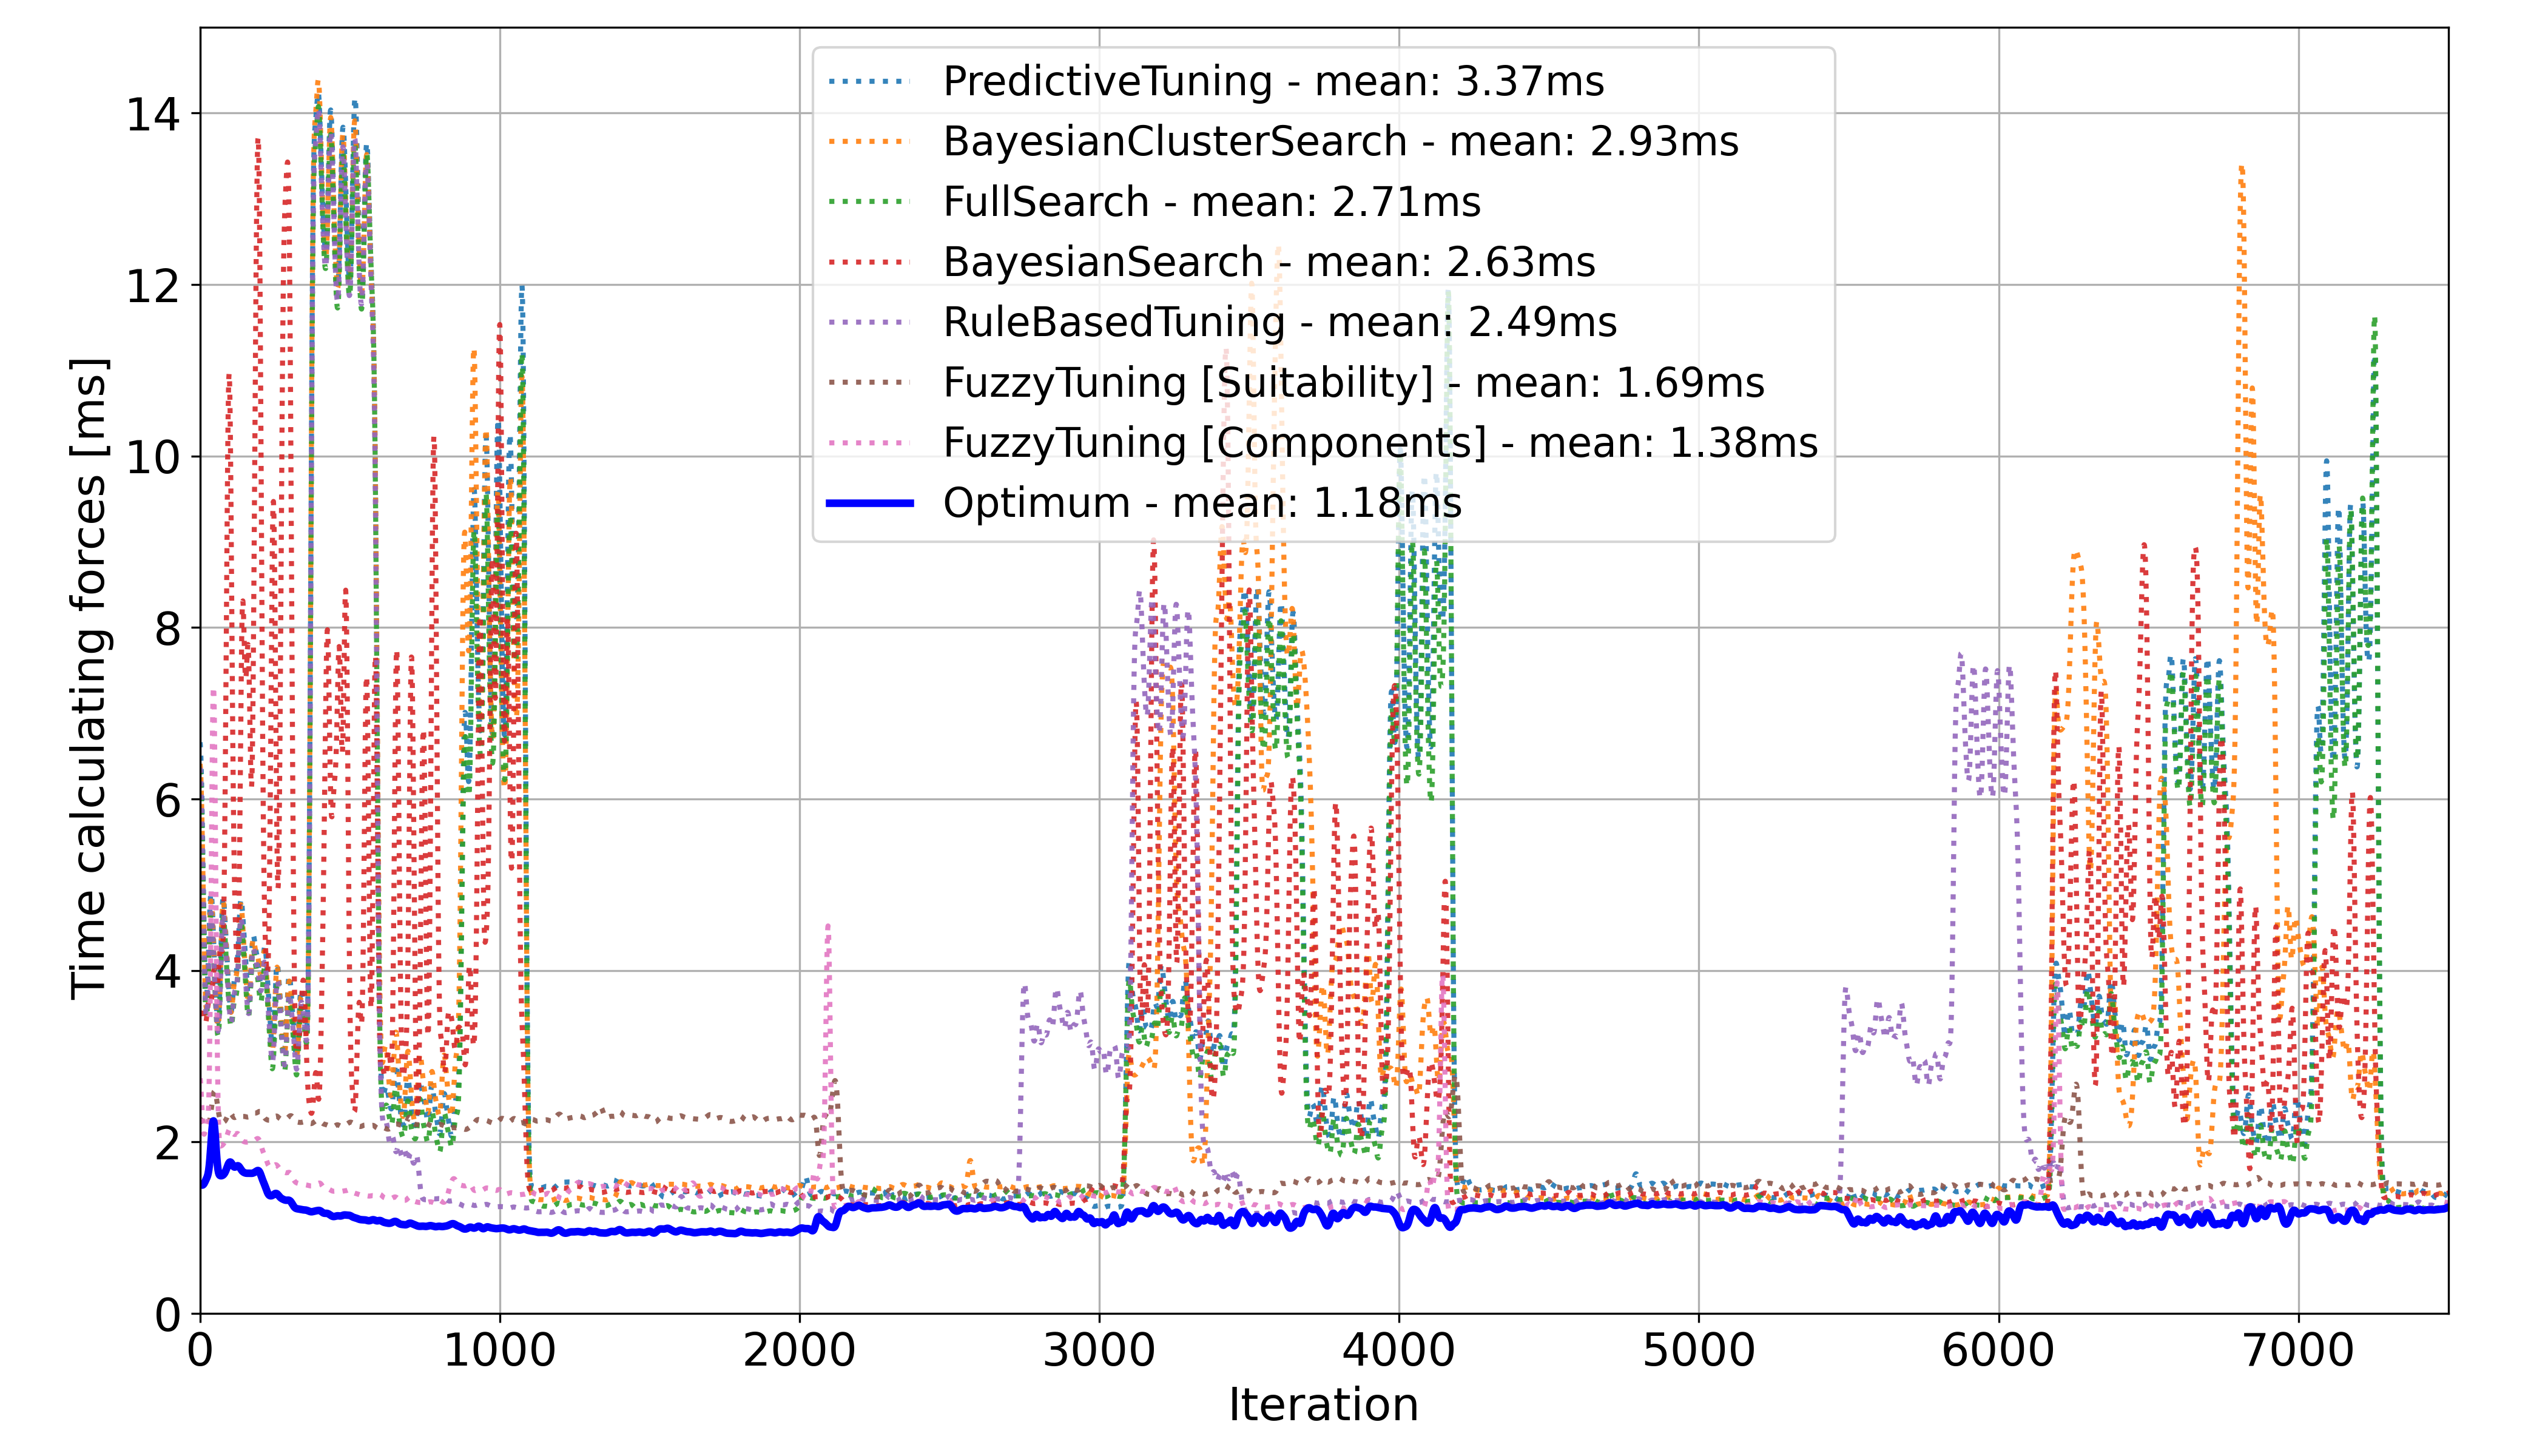
\includegraphics[width=\columnwidth]{figures/unnecessary-tuning-phases.png}
    \caption{
        Typical timing profile of the ExplodingLiquid simulation for every available tuning strategy. The plot clearly shows that all tuning strategies introduce overhead during the tuning phases. (Data obtained from \cite{lerchner2024})
    }
    \label{fig:unnecessary-tuning-phases}
\end{figure}

\section{Early Stopping Optimization}

To minimize some of the introduced drawbacks of the auto-tuning process, \cite{endreport.pdf}\cite{Manuel_Lerchner_Thesis.pdf}\cite{autopas_issue673} suggest that an \textit{early stopping} mechanism could be beneficial for the AutoPas framework. The primary goal of such a mechanism would be to detect tuning iterations that take much longer than the currently best-known configuration and to stop the evaluation of those configurations early. There are two approaches to this problem:


\begin{itemize}
    \item \textbf{Stopping Further Samples}\\
          As AutoPas evaluates a configuration multiple times to reduce measurement noise, a simple way to implement early stopping would be to stop the evaluation of further samples as soon as it is clear that the performance is significantly worse than the best-known configuration.

          This approach may not be as effective as it still requires fully evaluating the first sample of a bad configuration.
    \item \textbf{Interrupting the Evaluation}\\
          A more fine-grained approach, proposed in~\cite{endreport.pdf}, could interrupt the evaluation of a long-running configuration while it is still being evaluated.

          Implementing this approach would require a big rewrite of AutoPas' internal structure and is therefore not feasible in the short term.
\end{itemize}

To get a first impression of the potential benefits of an early stopping mechanism, we implemented the first approach into the AutoPas framework. The changes to the existing codebase are minimal, as the early-stopping mechanism can be implemented using existing functionality. \autoref{alg_early_stopping} shows the main changes to the \texttt{AutoTuner.cpp} file.

Both described approaches require a user-defined threshold for the $allowedSlowdownFactor$ that determines when the evaluation of a configuration should be stopped. As finding optimal thresholds is non-trivial and may depend on the simulation scenario and the tuning strategy, suitable thresholds will be determined empirically in \autoref{sec:evaluation}.

\begin{algorithm}[h]
    \small
    \caption{Early Stopping Algorithm in AutoPas}
    \label{alg_early_stopping}
    \begin{algorithmic}[1]
        \Procedure{evaluateConfiguration}{performance}
        \State $fastestTime \gets \min(fastestTime, performance)$
        \State $slowdownFactor \gets \frac{performance}{fastestTime}$
        \If{$slowdownFactor > allowedSlowdownFactor$}
        \State $abort \gets true$
        \EndIf
        \EndProcedure

        \vspace{0.5em}

        \Procedure{GetNextConfiguration}{}
        \If{not $inTuningPhase$}
        \State \Return ($currentConfig, false)$
            \ElsIf{$numSamples$ $<$ $maxSamples$ \redbox{\textbf{and} not $abort$}}
            \State \Return $(currentConfig, true)$
            \Else
            \State $stillTuning \gets \Call{tuneConfiguration}{~}$
            \State \Return $(newConfig, stillTuning)$
        \EndIf
        \EndProcedure
    \end{algorithmic}
\end{algorithm}

\subsection{Evaluation: Exploding Liquid Simulation}
\label{sec:evaluation}

To evaluate the performance of the early stopping mechanism, we perform a benchmark using the Exploding Liquid scenario provided by \texttt{md-flexible}. The simulation consists of 1764 initially close-packed particles, rapidly expanding outwards and eventually hitting the simulation boundaries. All benchmarks are performed on a single node of the \href{https://doku.lrz.de/coolmuc-2-11484376.html}{CoolMUC2} supercomputer using 14 threads. To ensure reproducibility, all runs are repeated three times.

\begin{description}[style=nextline]
    \item[FullSearch (\autoref{fig:full_search})]
        When using the early stopping optimization together with the FullSearch strategy, the total simulation time
        can be reduced from 36.22 seconds to 30.84 seconds at $allowedSlowdownFactor \approx4$. This results in a reduction of the total simulation time by 14.8\%.
    \item[PredictiveTuning (\autoref{fig:predictive_tuning})]
        When using the early stopping optimization together with the PredictiveTuning strategy, the total simulation time can be reduced from 28.62 seconds to 23.23 seconds at a $allowedSlowdownFactor \approx5$. This results in a reduction of the total simulation time by 18.9\%.
\end{description}

\begin{figure}[H]
    \centering

    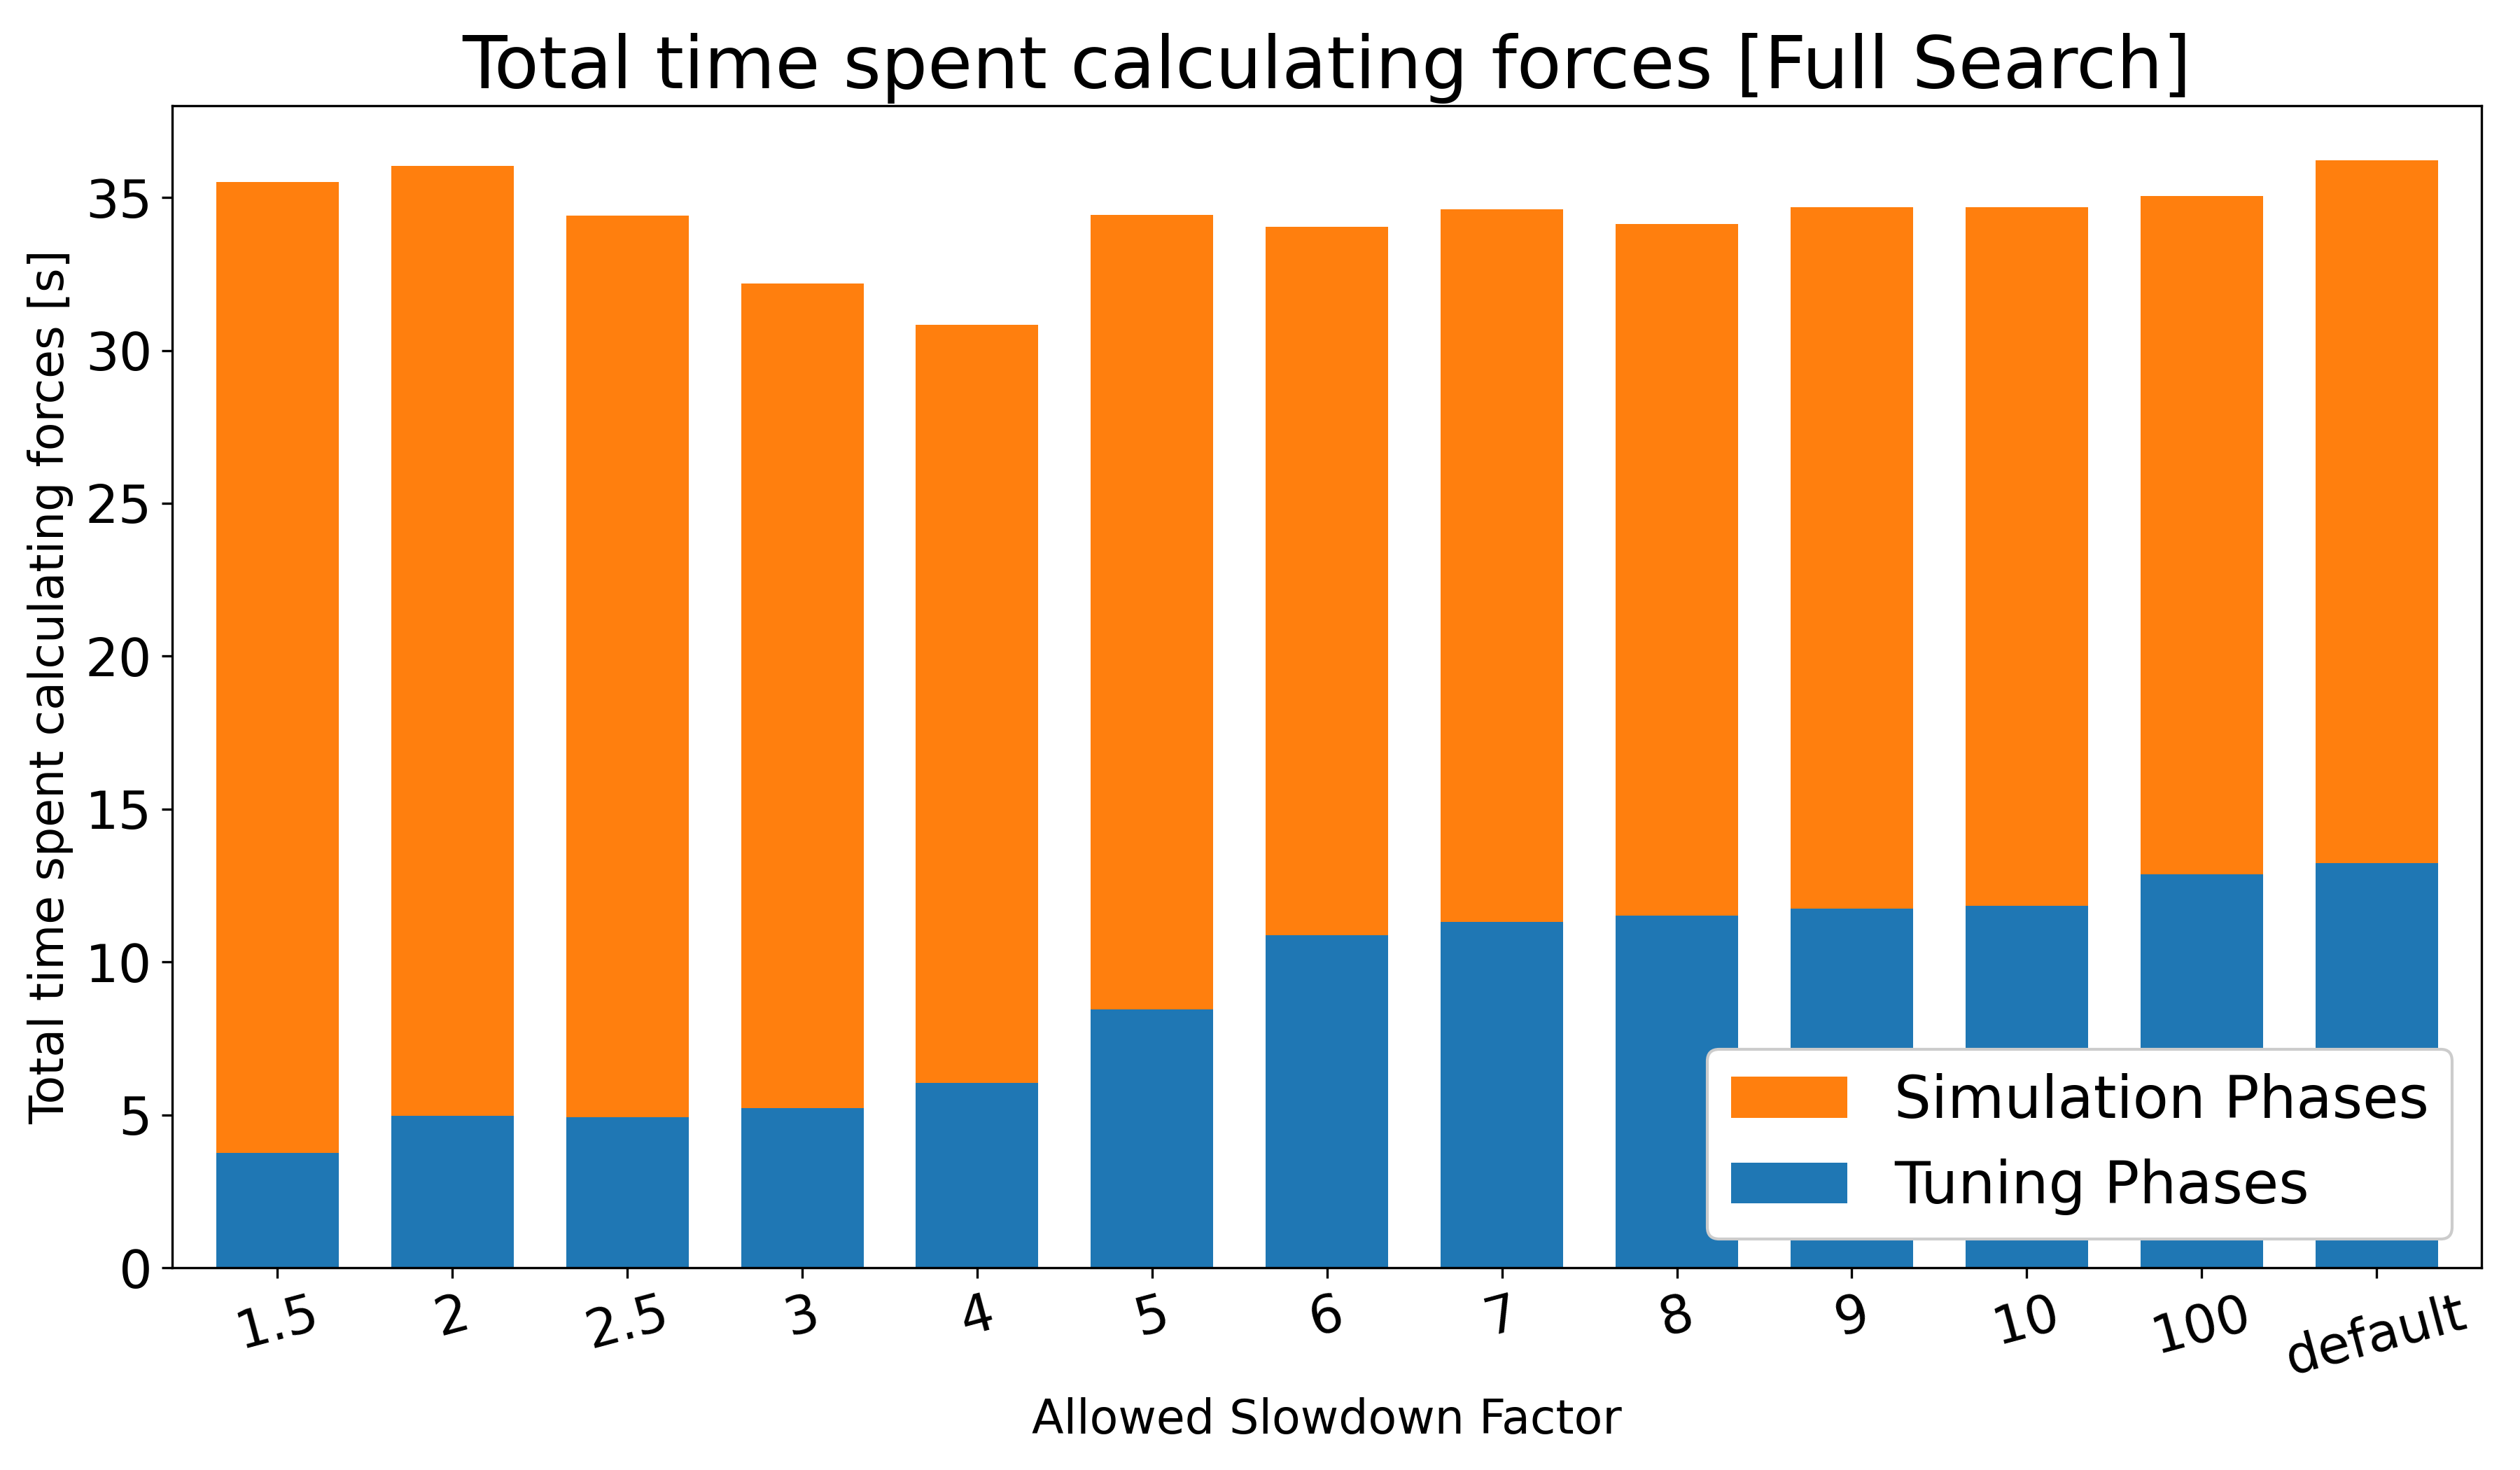
\includegraphics[width=\columnwidth]{../data/explodingLiquid/cluster/fullSearch/analytics/total_time_average.png}

    \caption{Total Simulation Time for Exploding Liquid Simulation for different values of $allowedSlowdownFactor$ using the FullSearch strategy with early stopping.}
    \label{fig:full_search}
\end{figure}

\begin{figure}[H]
    \centering

    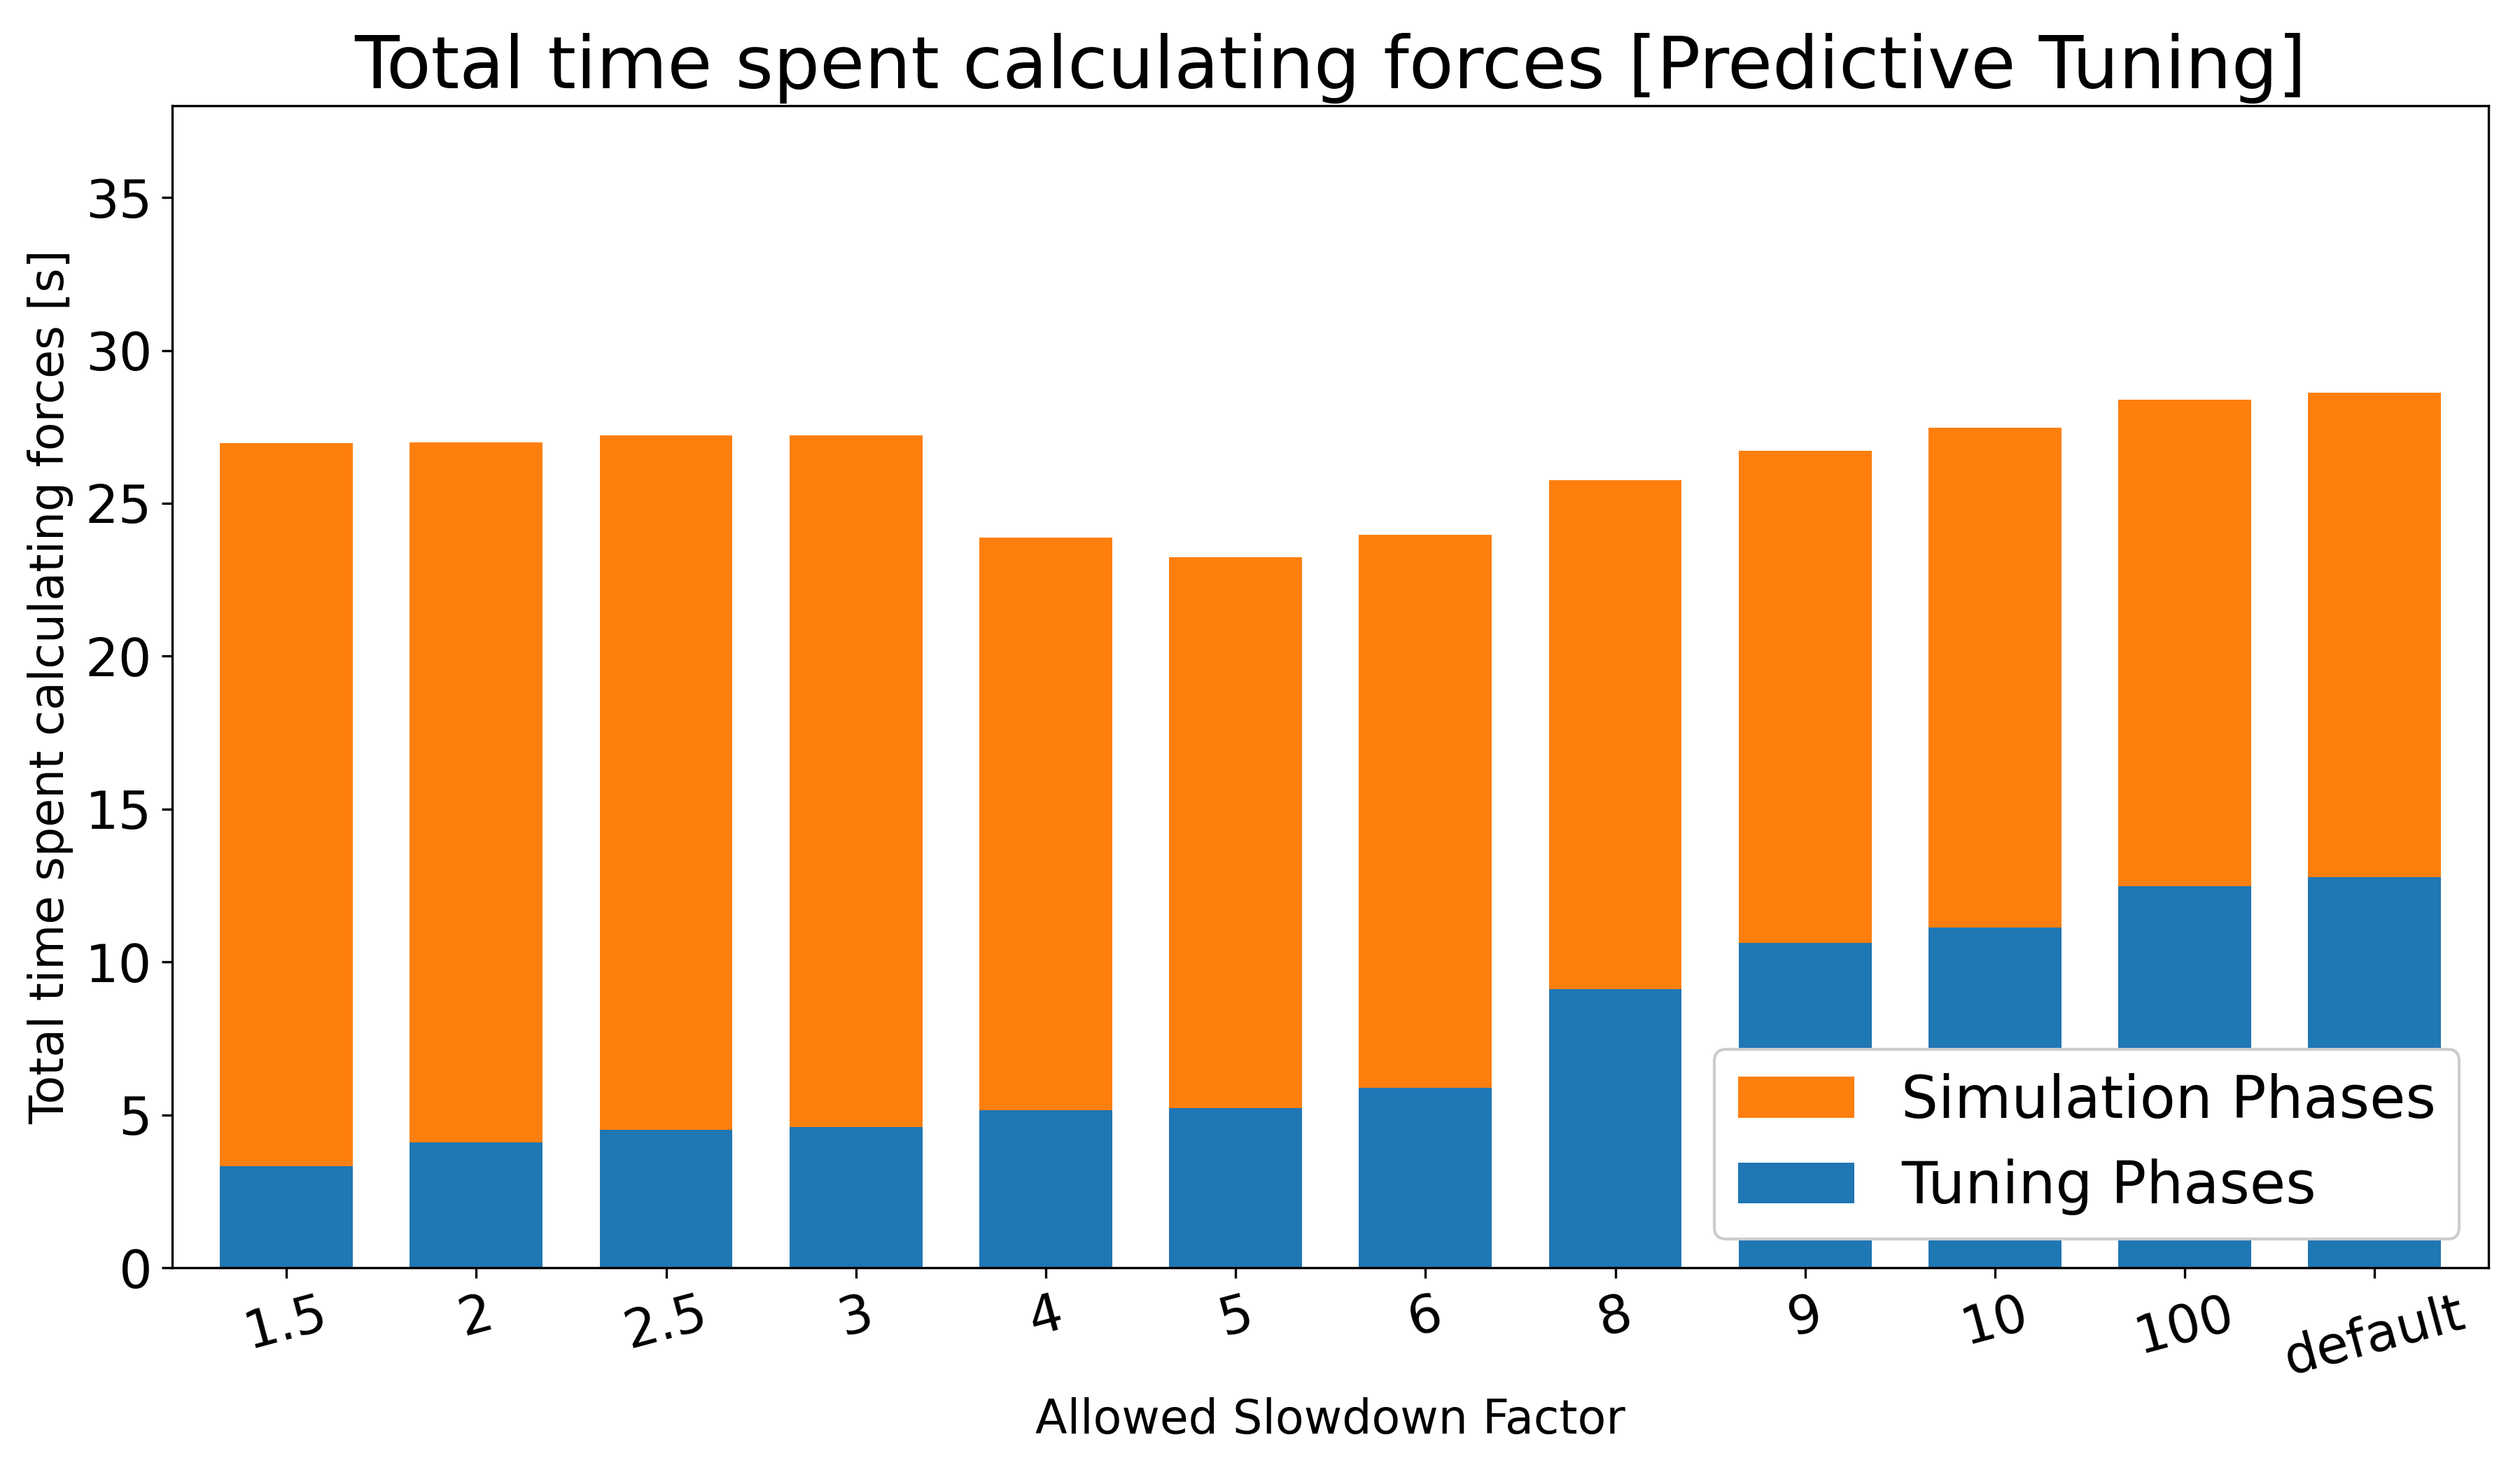
\includegraphics[width=\columnwidth]{../data/explodingLiquid/cluster/predictiveTuning/analytics/total_time_average.png}

    \caption{Total Simulation Time for Exploding Liquid Simulation for different values of $allowedSlowdownFactor$ using the PredictiveTuning strategy with early stopping.}
    \label{fig:predictive_tuning}
\end{figure}

\subsection{Analysis and Discussion}
\begin{description}[leftmargin=1.2em, font=\itshape]
    \item[Optimal Thresholds:]
        The evaluated benchmarks show that using the early stopping mechanism can reduce the total simulation time for both the FullSearch and PredictiveTuning strategies. However, there only exists a narrow range of $allowedSlowdownFactor$ values where the early stopping mechanism is beneficial. Outside of this range, the total simulation time is comparable to the performance of the simulation without the early stopping mechanism.

        This is expected, as both limiting cases result in undesirable behavior: $allowedSlowdownFactor \to 1$ results in tuning phases with very few samples per configuration, as even slight noise in the performance measurements causes the early stopping mechanism to abort a configuration. This prohibits a reasonable estimation of the performance of a configuration and could result in a suboptimal configuration winning the tuning phase. On the other hand, $allowedSlowdownFactor \to \infty$ results in the early stopping mechanism never aborting a configuration, which is equivalent to not using the early stopping mechanism at all. Picking a suitable threshold corresponds to finding a balance between the two extremes.

        From the executed benchmarks, we deduce that the optimal threshold for the early stopping mechanism is around 4-5 for the \textit{Exploding Liquid} scenario. However, the optimal threshold probably varies between different simulation scenarios and tuning strategies, and further benchmarks are required to determine the optimal threshold for other scenarios. It is, however, noteworthy that the early stopping mechanism never caused a significant increase in the total simulation time, even when using suboptimal thresholds.

    \item[Combination with Tuning Strategies:]
        The evaluated benchmarks show that a combination of the early stopping mechanism with good tuning strategies is beneficial and additionally reduces the total simulation time. Good tuning strategies are expected to benefit more from the early stopping mechanism, as evaluating good configurations early results in faster convergence of the $fastestTime$ variable. This allows for the early stopping mechanism to abort more configurations, further reducing the total tuning time.

    \item[Limitations and Future Work:]
        The current implementation of the early stopping mechanism resets the $fastestTime$ variable prior to each tuning phase, resulting in a complete loss of the information gathered in previous iterations. This ensures that the $fastestTime$ variable is always up-to-date with the current simulation state and prevents the early stopping mechanism from mistakenly aborting configuration based on a timing measurement that can no longer be achieved due to changes in the simulation state.

        An improved version could only reset the $fastestTime$ variable to a running average of timing measurements collected during the prior simulation phase. This would allow the early stopping mechanism to start with a reasonable estimate of achievable performance, increasing the likelihood of aborting unsuitable configurations early.

\end{description}

\section{Comparison with Other MD Engines}

Established MD engines such as GROMACS, LAMMPS, and ls1 mardyn have been developed over many years and have been optimized to achieve high performance in their respective use cases. This section provides a short overview of those engines and highlights the differences in their implementations.

\subsection{GROMACS}

Contrary to AutoPas, GROMACS only implements a single, highly optimized variant of the Verlet Cluster List algorithm. The algorithm allows for flexible cluster sizes specifically designed for achieving good SIMD vectorization~\cite{PALL20132641}.

Gromacs allows setting the vectorization parameters for the cluster size $M$ and the number of particles in neighbor groups $N$ statically to tune the force calculations to the SIMD width of the system~\cite{PALL20132641}. With suitable values for $M$ and $N$, computations of $M \times N$ particle interactions can be performed with just two SIMD load instructions~\cite{Solving_Software_Challenges_Exascale_2014}, drastically reducing the number of memory operations required for the force calculations and reaching up to 50\% of the peak flop rate on all supported hardware platforms~\cite{Solving_Software_Challenges_Exascale_2014}.

Gromacs defaults to $M=4$ and selects $N \in \{2, 4, 8\}$ depending on the SIMD width of the system. However, tuning those values is time-consuming and relies on a detailed understanding of many low-level software optimization aspects of the different hardware platforms~\cite{PALL20132641}. In GROMACS, the developers must manually create and maintain such performance models for each supported hardware platform, which is a time-consuming and labor-intensive process~\cite{PALL20132641}.

\subsection{LAMMPS}

LAMMPS utilizes a performance-optimized version of the Verlet List algorithm. To optimize cache performance, LAMMPS stores its neighbor lists in a global data structure split across multiple memory pages. Each page stores neighbor lists for multiple particles in a contiguous memory block, allowing for efficient allocation and deallocation of the neighbor lists~\cite{THOMPSON2022108171}. All particle data is stored in a Structure of Arrays (SoA) layout~\cite{THOMPSON2022108171}, allowing for efficient vectorization of the force calculations.

\subsection{ls1 mardyn}

ls1 mardyn differs from the previously mentioned MD engines as it uses the Linked Cells algorithm for particle interactions. Using LinkedCells provides a better memory efficiency than GROMACS and LAMMPS, allowing for simulations of massive particle systems~\cite{tchipev2019twe}. Internally, ls1 mardyn uses the default data layout of \textit{AoS} (Array of Structures) for storing particle data. However, particular branches aimed at simulating massive particle systems can use a \texttt{RMM} (Reduced Memory Mode) layout in combination with a \textit{SoA} (Structure of Arrays) data layout, allowing for simulations of up to twenty trillion atoms~\cite{tchipev2019twe}.

\section{Conclusion}

We presented an overview of the AutoPas framework and its auto-tuning capabilities and demonstrated the benefits and challenges of dynamic auto-tuning in molecular dynamics simulations.

Moreover, we investigated the potential of a naive early stopping mechanism to reduce some of the inherent overhead caused by tuning phases and demonstrated that such a mechanism can reduce the total simulation time by up to 18.9\% in specific scenarios.

The comparison with established MD engines such as GROMACS, LAMMPS, and ls1 mardyn reveals a fundamental trade-off in software design. While these engines achieve excellent performance through highly specialized implementations, AutoPas offers greater flexibility and adaptability through its modular architecture and dynamic optimization capabilities by accepting some performance overhead.\\
However, the successful integration of AutoPas into ls1 mardyn and LAMMPS demonstrates that these approaches can be complementary rather than mutually exclusive.

\newpage

\bibliographystyle{IEEEtran}
\bibliography{literature}


\end{document}

